\documentclass[11pt]{article}

\usepackage[utf8]{inputenc}
\usepackage[T1]{fontenc}
\usepackage{amsmath}
\usepackage[spanish,es-noindentfirst]{babel}
\usepackage{graphicx}
\usepackage{booktabs}
\usepackage{tabularx}
\usepackage{array}
\usepackage{geometry}
\usepackage[table]{xcolor}
\usepackage{titlesec}
\usepackage{caption}
\usepackage{float}
\usepackage[hidelinks]{hyperref}

\geometry{a4paper, top=2.4cm, bottom=2.6cm, left=2.4cm, right=2.4cm}

% ------- Paleta de colores del documento -------
\definecolor{usblue}{RGB}{23,55,94}
\definecolor{usaccent}{RGB}{0,124,146}
\definecolor{usgrey}{RGB}{90,100,110}
\definecolor{tablehead}{RGB}{23,55,94}
\definecolor{tablerow}{RGB}{238,242,246}

\hypersetup{colorlinks=true, linkcolor=usblue, urlcolor=usaccent}

\titleformat{\section}
  {\Large\bfseries\color{usblue}}{\thesection}{0.6em}{}
\titleformat{\subsection}
  {\large\bfseries\color{usaccent}}{\thesubsection}{0.6em}{}
\titleformat{\subsubsection}
  {\normalsize\bfseries\color{usgrey}}{\thesubsubsection}{0.6em}{}

\captionsetup{font=small, labelfont={bf,color=usblue}}
\renewcommand{\arraystretch}{1.2}
\setlength{\tabcolsep}{5pt}

\newcommand{\urlt}{\texttt}
\newcommand{\code}[1]{\texttt{#1}}

\begin{document}

%======================================================================
%  PORTADA
%======================================================================
\begin{titlepage}
\centering
{\color{usblue}\rule{\textwidth}{2pt}}\\[0.6cm]
{\Huge\bfseries\color{usblue} UrbanSafe AI}\\[0.35cm]
{\LARGE Ecosistema de Movilidad Predictiva y Segura}\\[0.25cm]
{\large\color{usgrey} Deliverable 1 --- Integrated Project Definition}\\[2.1cm]

\begin{minipage}{0.8\textwidth}
\centering
{\bfseries Curso:} Desarrollo de Productos de Datos (DS-3022) --- UTEC\\[2pt]
{\bfseries Ciclo:} 2026-II \quad\textbar\quad {\bfseries Semana de entrega:} 07 (23 de septiembre de 2026)\\[2pt]
{\bfseries Equipo:} Elmer Jose Manuel Villegas Suarez | Alessandro Facundo Freed Monzón Gallegos | Juan David Velo Poma (Líder)\\[8pt]
{\bfseries Alcance:} Definición del problema, requisitos, arquitectura, EDA, selección de modelos y prototipo de baja fidelidad.
\end{minipage}\\[1.8cm]

{\color{usblue}\rule{\textwidth}{2pt}}
\end{titlepage}

\tableofcontents
\newpage

%======================================================================
\section{Resumen ejecutivo}
\label{sec:resumen}
%----------------------------------------------------------------------
UrbanSafe AI es un producto de datos orientado al Sistema Integrado de Transporte de Lima
Metropolitana (Metropolitano y Corredores Complementarios). Su objetivo central es \textbf{reducir
los tiempos de espera y la incertidumbre de los pasajeros} en estaciones y paraderos, mostrando el
\textbf{aforo proyectado} de las próximas unidades y su \textbf{tiempo estimado de llegada (ETA)},
y recomendando de forma prescriptiva si el usuario debe \textbf{abordar, esperar la siguiente unidad
o cambiar de paradero}. Como funcionalidad secundaria, incorpora un módulo de \textbf{enrutamiento
peatonal seguro} (primera y última milla) que prioriza vías iluminadas y vigiladas sobre la
distancia más corta.

El proyecto evoluciona de la \emph{Hackathon ATU 2026} y del concepto \emph{Urbyte}. Combina fuentes
de datos abiertos (validaciones de transporte, telemetría de tráfico, OpenStreetMap y clima) con una
capa sintética de congestión y aforo para resolver el problema de arranque en frío.

\paragraph{Estado del avance (S07).} Este entregable consolida la \textbf{Fase 1 --- Definición e
Integración de Requerimientos}: especificación de requisitos funcionales y no funcionales, casos de
uso, análisis exploratorio de datos (EDA), selección justificada de modelos y prototipo de baja
fidelidad. La demanda base prevista es la de la \textbf{ATU de Lima} (solicitada y pendiente de
respuesta); como proxy de la misma naturaleza BRT se usa el dataset de \textbf{Validaciones
Troncales de TransMilenio (Bogotá)}.

%======================================================================
\section{Problema y propuesta de valor}
\label{sec:problema}
%----------------------------------------------------------------------
\subsection{Contexto y problemática}
En el Sistema Integrado de Transporte de Lima los usuarios enfrentan alta incertidumbre respecto a
los \textbf{tiempos de llegada} y al \textbf{nivel de aforo} (asientos disponibles, de pie o bus
saturado) de las unidades, lo que genera tiempos de espera ineficientes, viajes incómodos y
aglomeraciones severas en paraderos.

A esta ineficiencia se suma la problemática de seguridad ciudadana en la \emph{primera y última
milla} (tramos a pie desde el origen hacia el paradero y desde la estación hacia el destino). Según
el INEI (2025), la percepción de inseguridad en las principales áreas urbanas supera el 85\%, con
mayor incidencia de robos y hurtos en vías desoladas o mal iluminadas. Las herramientas de
navegación convencionales optimizan por distancia o tiempo mínimo, ignorando el riesgo peatonal y el
estado de ocupación de las unidades.

\subsection{Propuesta de valor}
\begin{itemize}
  \item \textbf{Predictiva:} inferencia del aforo futuro de las unidades ({\normalfont\emph{Asientos /
        De pie / Saturado}}) y del ETA de las dos próximas unidades, reduciendo la permanencia en el andén.
  \item \textbf{Prescriptiva:} matriz de decisión que recomienda abordar, esperar el siguiente servicio
        o cambiar de paradero, con nivel de confianza y banda de incertidumbre.
  \item \textbf{Seguridad peatonal:} enrutamiento por índice de riesgo urbano para la primera y última
        milla, con comparación contra la ruta más corta y tolerancia de caminata ajustable.
\end{itemize}

\subsection{Fuentes de datos}
\begin{table}[H]
\centering
\caption{Fuentes de datos del producto.}
\label{tab:fuentes}
\begin{tabularx}{\textwidth}{l>{\raggedright\arraybackslash}X}
\toprule
\textbf{Fuente} & \textbf{Rol en el producto} \\
\midrule
\textbf{Validaciones ATU (ProTransporte)} & Demanda base prevista --- \emph{solicitud pendiente}.
Mientras tanto se usa como proxy el dataset de Validaciones Troncales de TransMilenio (Bogotá),
misma naturaleza BRT. \\
\textbf{TomTom Traffic API} & Telemetría de congestión en tiempo real (key \code{TOMMTOM\_KEY} en
\code{.env}); feature de retraso del bus. Sin key, el sistema opera en \emph{Modo Histórico} (RF-05). \\
\textbf{OpenStreetMap (OSM)} & Infraestructura urbana (luminarias, comisarías, comercios, red vial)
$\rightarrow$ índice de seguridad peatonal (segundo plus). \\
\textbf{Meteostat} & Clima horario de Bogotá --- \textbf{solo EDA}; no entra a los predictores. \\
\textbf{Dataset sintético} & Capa de congestión (\code{congestion\_sintetica.csv}) y simulación de
aforo para el arranque en frío. \\
\bottomrule
\end{tabularx}
\end{table}

%======================================================================
\section{Data Product Canvas}
\label{sec:canvas}
%----------------------------------------------------------------------
El lienzo del producto de datos define la propuesta de valor, los clientes y usuarios, las fuentes de
datos, las decisiones soportadas y el modelo de negocio del producto.

\begin{figure}[H]
\centering
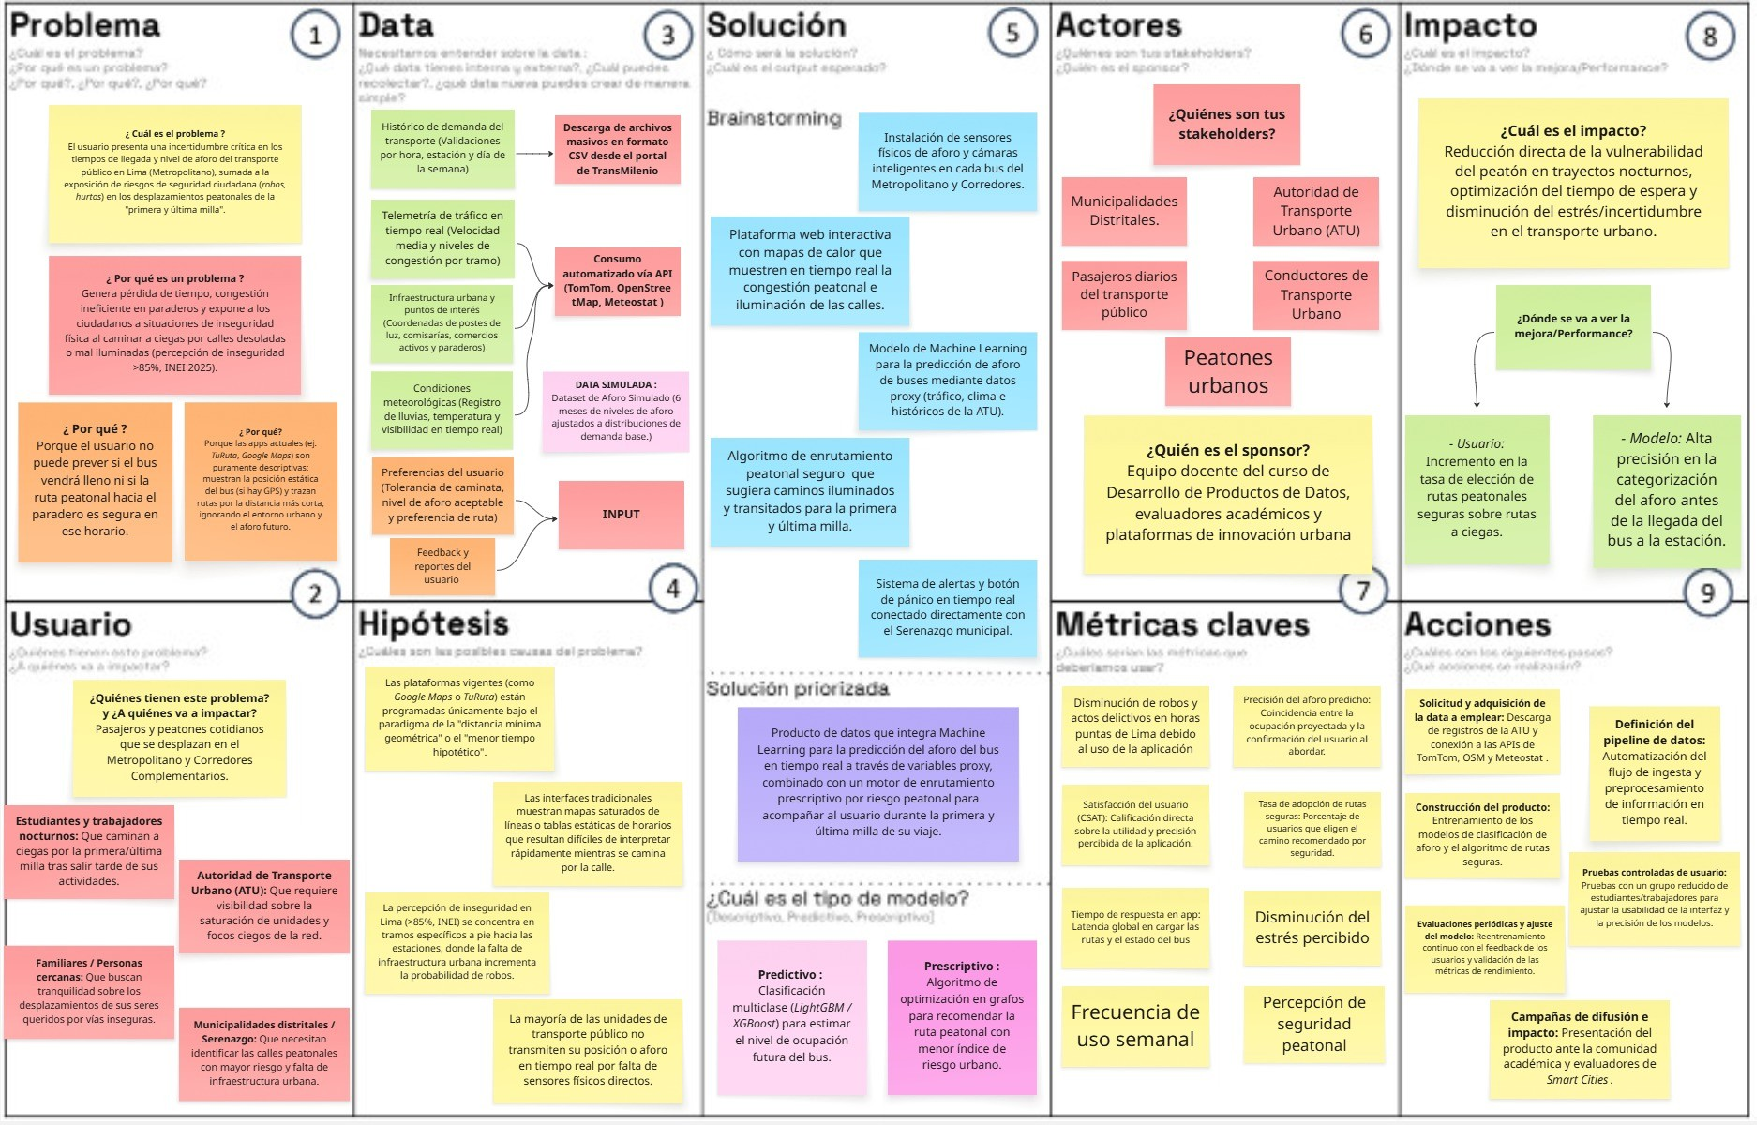
\includegraphics[width=\textwidth]{../DataProductCanvas.pdf}
\caption{Lienzo del Producto de Datos (imagen integrada de la entrega).}
\label{fig:canvas}
\end{figure}

\subsection{Usuarios objetivo y stakeholders}
\begin{description}
  \item[Usuarios del transporte público (pasajeros y peatones):] planifican sus viajes reduciendo la
        incertidumbre del aforo, optimizando sus tiempos de espera y transitando por caminos peatonales
        con menor exposición a la delincuencia.
  \item[Planificadores urbanos y entidades reguladoras (ATU y municipios):] aprovechan el análisis
        agregado de la demanda e identifican zonas críticas de la primera y última milla.
\end{description}

\begin{table}[H]
\centering
\caption{Mapa de stakeholders y actores.}
\label{tab:stakeholders}
\begin{tabularx}{\textwidth}{llc}
\toprule
\textbf{Stakeholder / Actor} & \textbf{Categoría} & \textbf{Impacto / Poder} \\
\midrule
Pasajeros y peatones urbanos & Actor primario & Alto / Alto \\
Familiares y red de apoyo & Beneficiario indirecto & Medio / Bajo \\
Autoridad de Transporte Urbano (ATU) & Aliado estratégico & Alto / Medio \\
Municipalidades distritales / Serenazgo & Stakeholder operativo & Medio / Medio \\
Conductores y operadores de bus & Stakeholder indirecto & Medio / Bajo \\
\bottomrule
\end{tabularx}
\end{table}

%======================================================================
\section{Requerimientos y casos de uso}
\label{sec:req}
%----------------------------------------------------------------------
\subsection{Historias de usuario y job stories}
\begin{itemize}
  \item \textbf{US-01 (Núcleo):} como pasajero en hora punta, quiero consultar la categoría de
        ocupación proyectada del próximo bus antes de que llegue, para decidir si me preparo para subir,
        espero la siguiente unidad o camino a otro paradero.
  \item \textbf{US-02:} como usuario en el andén, quiero comparar el tiempo de llegada y el aforo del
        bus actual frente al siguiente, para elegir la alternativa más cómoda y rápida.
  \item \textbf{US-03:} como usuario que acaba de abordar, quiero confirmar con un toque si la
        estimación de aforo fue acertada (retroalimentación del modelo).
  \item \textbf{US-04 (Segundo plus):} como peatón, quiero una ruta guiada por calles iluminadas y
        transitadas para reducir mi exposición a zonas con riesgo delictivo.
\end{itemize}

\subsection{Casos de uso principales}
\subsubsection{UC-01 --- Inferencia de aforo predictivo multiclase (núcleo)}
\begin{description}
  \item[Actores:] Pasajero/peatón (principal); APIs y modelo ML (secundarios).
  \item[Disparador:] el usuario selecciona servicio, ruta y estación de abordaje.
  \item[Flujo principal:] (1) se ingiere velocidad y congestión de TomTom Traffic; (2) se cruza con el
        histórico horario de validaciones; (3) el modelo clasifica el aforo en \emph{Asientos
        disponibles / De pie / Saturado}; (4) la interfaz muestra el aforo, su intervalo de confianza y
        el ETA.
  \item[Flujo alternativo:] si TomTom supera el timeout (2 s), el backend conmuta a inferencia basada
        en el histórico (respuesta con banner de \emph{Modo Histórico}).
\end{description}

\subsubsection{UC-02 --- Optimización prescriptiva de ruta peatonal segura}
Se carga el subgrafo peatonal OSM, se asigna a cada tramo un costo ponderado
$\text{Costo} = \text{Distancia} \times \text{Penalización}(\text{FaltaLuz},\,\text{FaltaComercios},\,
\text{DistanciaComisaria})$ y se calcula la trayectoria de costo mínimo con Dijkstra/A*: la app
presenta la ruta segura frente a la ruta geométrica más corta.

\subsection{Requerimientos funcionales (RF)}
\begin{table}[H]
\centering
\caption{Requerimientos funcionales.}
\label{tab:rf}
\begin{tabularx}{\textwidth}{ll>{\raggedright\arraybackslash}X}
\toprule
\textbf{ID} & \textbf{Módulo} & \textbf{Descripción} \\
\midrule
RF-01 & Núcleo & Mostrar el nivel de ocupación esperado de la próxima unidad en tres estados:
Asientos disponibles / viaje de pie / saturado. \\
RF-02 & Núcleo & Calcular el tiempo estimado de espera (min) de las dos próximas unidades. \\
RF-03 & Núcleo & Indicar si la opción más eficiente es abordar, esperar la siguiente o cambiar de paradero. \\
RF-04 & Núcleo & Feedback de un solo toque para confirmar la estimación al abordar. \\
RF-05 & Núcleo & Modo resiliente: ante caída de la API (TomTom), degradar a la matriz histórica de la ATU. \\
RF-06 & Peatonal & Computar un score de riesgo por tramo vial (alumbrado, comisarías, comercios, paraderos). \\
RF-07 & Peatonal & Generar la ruta peatonal prescriptiva y compararla con la ruta más corta geométrica. \\
RF-08 & Peatonal & Selector de tolerancia a caminata adicional para mayor seguridad. \\
\bottomrule
\end{tabularx}
\end{table}

\subsection{Requerimientos no funcionales (RNF)}
\begin{table}[H]
\centering
\caption{Requerimientos no funcionales.}
\label{tab:rnf}
\begin{tabularx}{\textwidth}{ll>{\raggedright\arraybackslash}X}
\toprule
\textbf{ID} & \textbf{Ámbito} & \textbf{Descripción} \\
\midrule
RNF-01 & Precisión analítica & Accuracy $\geq 75\%$ y F1-macro $\geq 0.72$ en prueba. \\
RNF-02 & Latencia global & Consulta de aforo y rutas en $\leq 2.0$ s en el percentil 95 (4G/5G). \\
RNF-03 & Disponibilidad & $\geq 99.0\%$ dentro del horario operativo (05:00--23:30). \\
RNF-04 & Ergonomía móvil & Operación con una sola mano, paleta de alto contraste nocturno, $\leq 2$ toques para el resultado. \\
RNF-05 & Gobernanza y privacidad & Sin geolocalización continua ni datos identificables; coordenadas de consulta efímeras (Ley N.° 29733). \\
\bottomrule
\end{tabularx}
\end{table}

\subsection{Criterios de aceptación (DoD)}
\begin{table}[H]
\centering
\caption{Criterios de aceptación.}
\label{tab:ac}
\begin{tabularx}{\textwidth}{ll>{\raggedright\arraybackslash}X}
\toprule
\textbf{ID} & \textbf{Requiere} & \textbf{Criterio} \\
\midrule
AC-01 & Pipeline & Integración automatizada de ATU, TomTom y OSM sin quiebre de esquema. \\
AC-02 & Aforo & Clasificador multiclase con F1 $\geq 0.72$ en las tres categorías (test independiente). \\
AC-03 & Espera & Recomendar abordar/esperar/cambiar con exactitud $\geq 80\%$ en casos evaluados. \\
AC-04 & Respuesta & Consulta integral en $\leq 2.0$ s (P95). \\
AC-05 & Grafo peatonal & Rutas con menor score de riesgo que la más corta en $\geq 80\%$ de casos. \\
AC-06 & Usabilidad & $\geq 60\%$ de usuarios declaran menor tiempo de espera percibido. \\
\bottomrule
\end{tabularx}
\end{table}

%======================================================================
\section{Arquitectura del sistema}
\label{sec:arquitectura}
%----------------------------------------------------------------------
El diagrama de arquitectura del sistema (Figura~\ref{fig:system}) define los componentes previstos:
ingesta de datos externos, capa de almacenamiento, pipeline de preprocesamiento, los modelos de cada
módulo y la interfaz de usuario.

\begin{figure}[H]
\centering
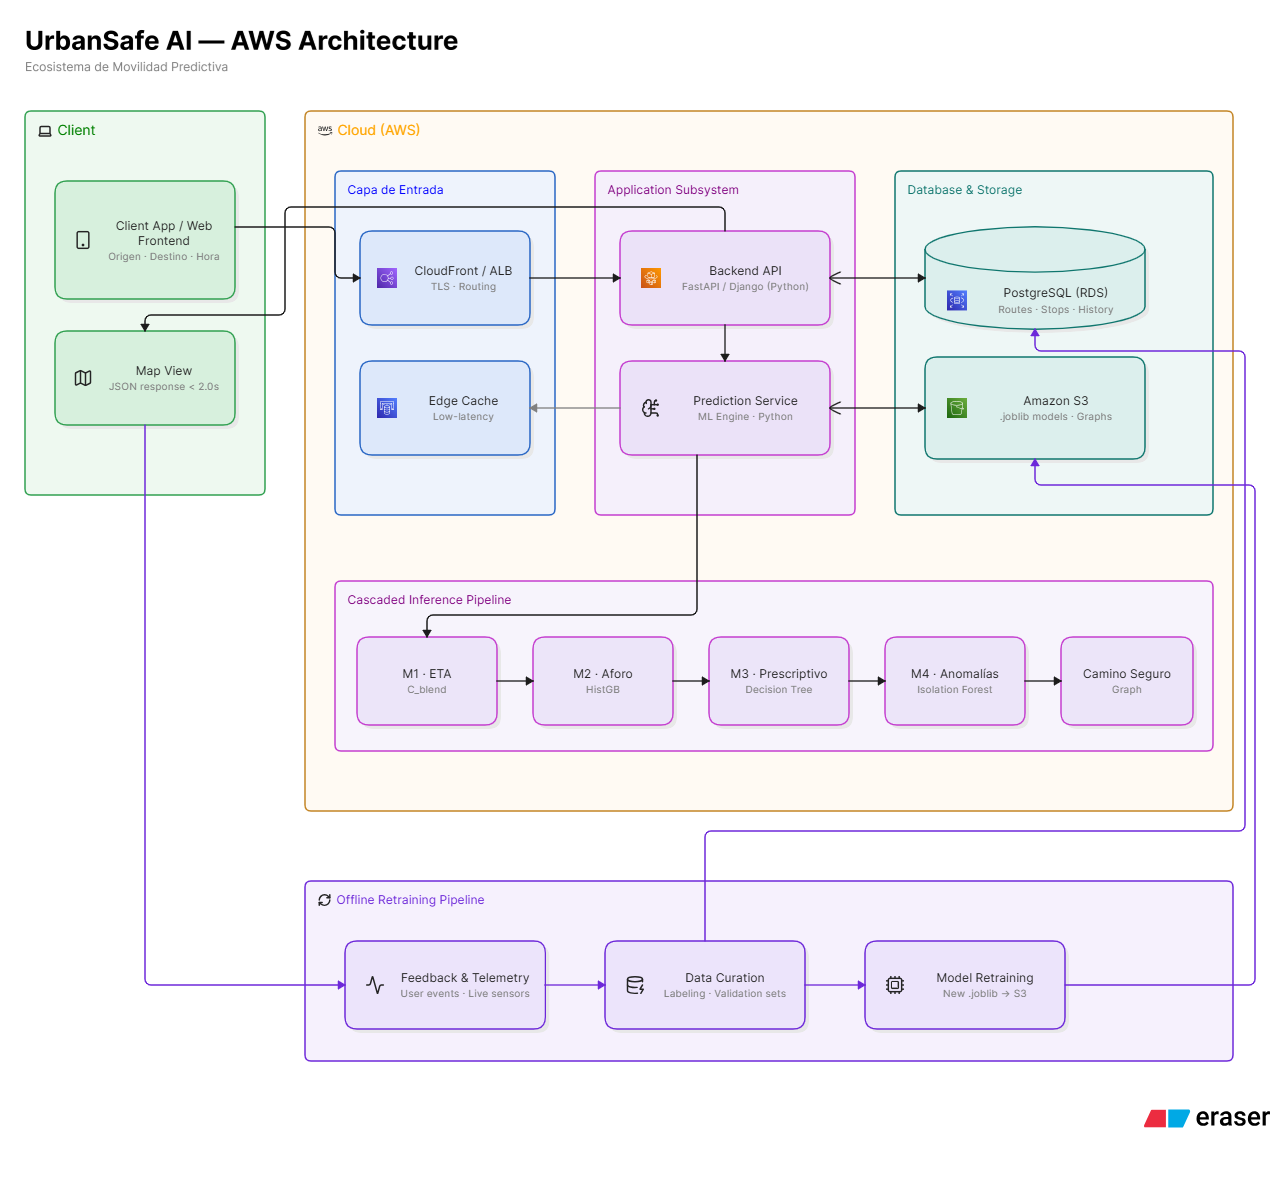
\includegraphics[width=\textwidth]{../system_diagram.png}
\caption{Diagrama de arquitectura del sistema UrbanSafe AI.}
\label{fig:system}
\end{figure}

\begin{itemize}
  \item \textbf{Capa de datos:} fuentes Open Data (TransMilenio/ATU, TomTom, OSM, Meteostat) y dataset
        sintético de congestión.
  \item \textbf{Capa de procesamiento:} scripts de descarga idempotentes y notebooks EDA que producen
        el dataset limpio de modelado.
  \item \textbf{Capa analítica:} cascada de inferencia (Chronos $\rightarrow$ ETA $\rightarrow$ Aforo
        $\rightarrow$ Recomendación) más detector de anomalías.
  \item \textbf{Capa de producto:} API REST (FastAPI) y app móvil con estados de degradación.
\end{itemize}

%======================================================================
\section{Workflow de la consulta principal}
\label{sec:workflow}
%----------------------------------------------------------------------
La Figura~\ref{fig:workflow} ilustra el flujo de la consulta principal: desde la selección del
usuario hasta la respuesta del sistema.

\begin{figure}[H]
\centering
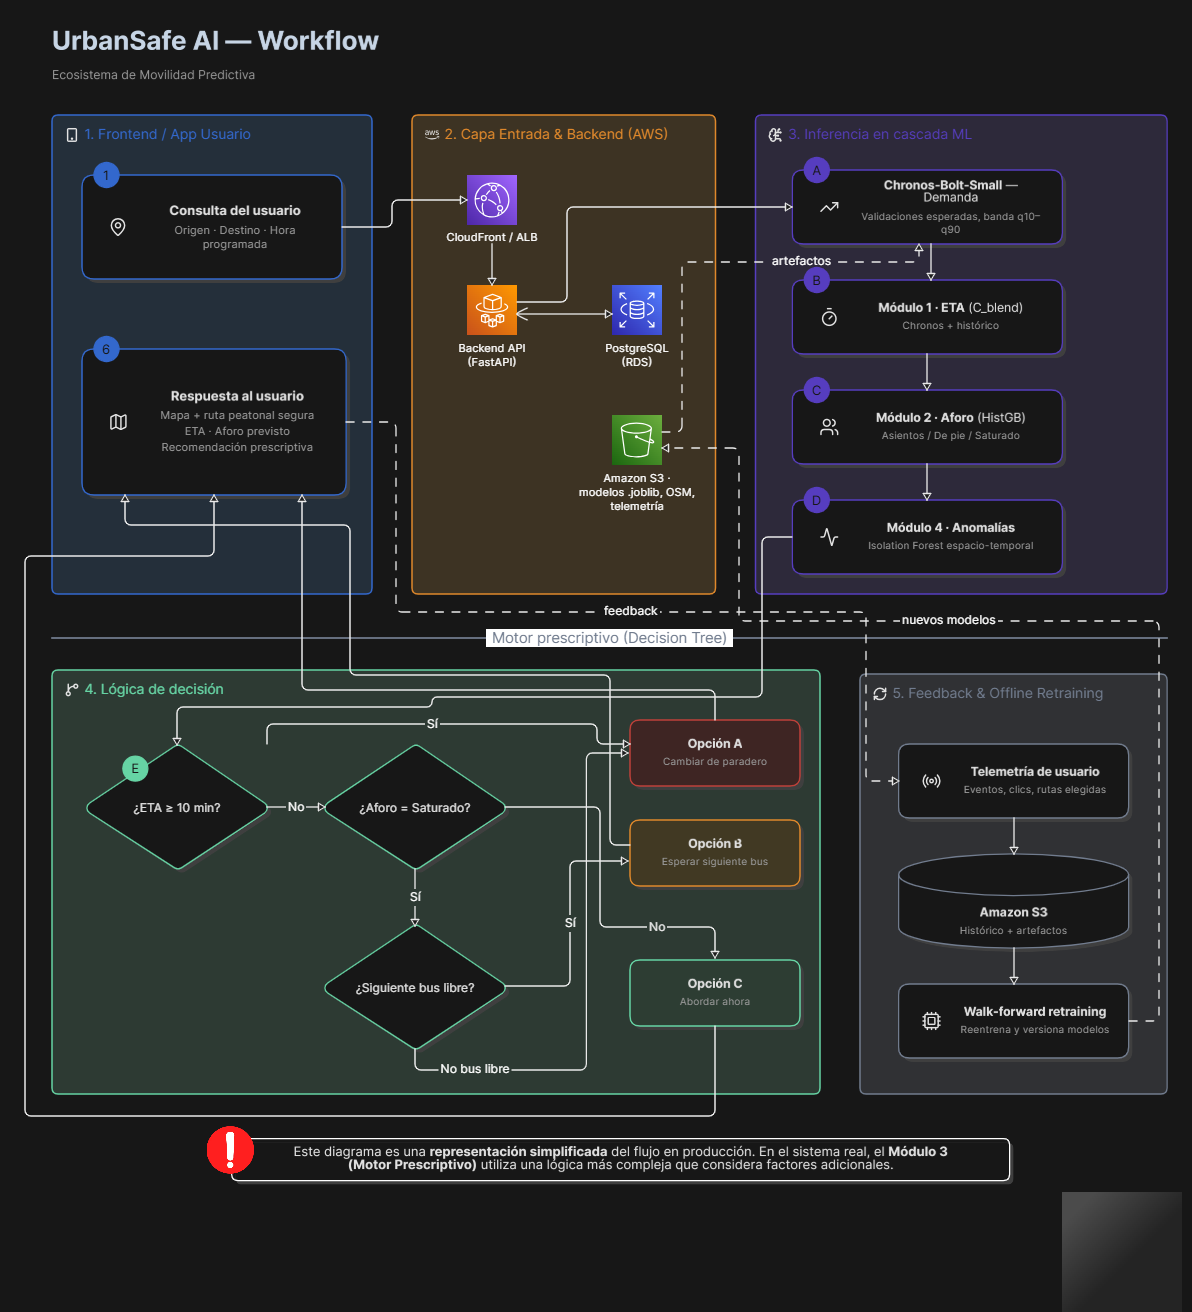
\includegraphics[width=0.95\textwidth]{../workflow.png}
\caption{Workflow de la consulta principal (aforo + ETA + recomendación).}
\label{fig:workflow}
\end{figure}

\subsection{Flujo petición -- respuesta}
\begin{enumerate}
  \item \textbf{Usuario (app móvil, 2 toques):} selecciona servicio (Metropolitano / Corredor),
        ruta y estación de abordaje. Declaración de uso efímero de ubicación (RNF-05).
  \item \textbf{Petición HTTP} a la API REST: \code{/consulta \{servicio, ruta, estacion, hora\}}.
  \item \textbf{Cascada de inferencia} (presupuesto P95 $\leq$ 2 s):
        \begin{enumerate}
          \item \emph{Pronóstico:} Chronos-Bolt-Small (fundacional, cero-tuning, CPU) pronostica las
                validaciones de la estación con banda de incertidumbre q10--q90.
          \item \emph{Módulo 1 --- ETA:} blend $C = w\cdot(\text{Chronos}) +
                (1-w)\cdot(\text{histórico por estación/hora})$, ajustado $\times$1.1 (ocupación media)
                o $\times$1.3 (alta); ETA de las 2 próximas unidades.
          \item \emph{Módulo 2 --- Aforo:} HistGB clasifica en Asientos / De pie / Saturado usando
                features de calendario, identidad de estación y validaciones pronosticadas.
          \item \emph{Módulo 4 --- Anomalías:} Isolation Forest vigila el corredor (drift) sin bloquear
                la respuesta.
          \item \emph{Módulo 3 --- Recomendación:} Tree aplica la matriz $U(\text{ETA},\,\text{Aforo})$:
                \begin{itemize}
                  \item ETA $\geq$ 10 min $\rightarrow$ \textit{cambiar de paradero};
                  \item ETA $<$ 10 min y bus saturado $\rightarrow$ \textit{esperar siguiente} si el
                  siguiente no viene saturado; si también viene lleno $\rightarrow$ \textit{cambiar de paradero};
                  \item en otro caso $\rightarrow$ \textit{abordar ahora}.
                \end{itemize}
        \end{enumerate}
  \item \textbf{Fallback (Modo Histórico, RF-05):} si la telemetría externa supera el timeout o no
        hay API key, la estimación se degrada a la matriz histórica de validaciones/headway, con banner
        informativo en la respuesta.
  \item \textbf{Respuesta JSON:} aforo con confianza e intervalo, ETA de las 2 unidades (rango, p. ej.
        3--5 min y 9--12 min), recomendación y banner de Modo Histórico si aplica.
  \item \textbf{Feedback (RF-04):} el usuario toca \emph{``Ya abordé este bus''} y marca la categoría
        real; el dato se persiste como ground-truth para reentrenamiento.
\end{enumerate}

%======================================================================
\section{Análisis exploratorio de datos (EDA)}
\label{sec:eda}
%----------------------------------------------------------------------
\subsection{Panorama del dataset}
\begin{table}[H]
\centering
\caption{Vista global del dataset (62 días, julio--agosto 2026).}
\label{tab:eda_resumen}
\begin{tabularx}{\textwidth}{ll}
\toprule
\textbf{Métrica} & \textbf{Valor} \\
\midrule
Filas del dataset limpio & 176,783 $\times$ 28 \\
Validaciones totales & 88,884,983 \\
Estaciones & 153 códigos Tullave (156 nombres) \\
Días / troncales / líneas & 62 / 12 / 13 \\
\emph{Dia 1} (hábil) vs \emph{Dia 2} (domingo/festivo) & 94\% / 6\% \\
Demanda en franjas pico & 62\% (pico AM 32.5\% + pico PM 29.2\%) \\
Estaciones sobre capacidad en su hora pico & 133 de 153 ($>$100\%) \\
\bottomrule
\end{tabularx}
\end{table}

\subsection{Principales hallazgos}
\begin{enumerate}
  \item \textbf{Estacionalidad fuerte:} `DiaSemana`, `Es\_Habil` y `Hora` explican la mayor parte de la
        varianza; la hora es la dimensión más predictiva.
  \item \textbf{Doble pico} (AM 05--09 h, PM 16--21 h) con forma distinta en domingo (un solo pico
        vespertino): se particiona por `Franja` y `Tipo\_Dia\_ok`.
  \item \textbf{Festivos mal etiquetados} en la fuente (4 festivos como \emph{Dia 1}): se corrigen con
        `Es\_Festivo` y `Tipo\_Dia\_ok`; los splits temporales aíslan días singulares.
  \item \textbf{La oferta sigue a la demanda} (corr. Frecuencia--Validaciones $=$ 0.498); `Frecuencia`
        y `N\_Rutas` correlacionan 0.92 (multicolinealidad a vigilar).
  \item \textbf{Ocupación proxy:} `Ocupacion\_pk = Validaciones / Cap\_total` (corr. 0.94 con
        `Validaciones`), base de la etiqueta de aforo.
  \item \textbf{Saturación generalizada:} 133/153 estaciones superan el 100\% de capacidad en su hora
        más cargada.
  \item \textbf{El clima es despreciable:} lluvia ligera asociada a $-$3\% (dentro del ruido), todas las
        correlaciones $|r| \leq 0.10$ a igual franja; la señal de temperatura es un proxy del ciclo
        horario. \textbf{El clima queda excluido del feature store.}
  \item \textbf{Cobertura incompleta:} ~5\% de filas sin oferta GTFS (flag `Sin\_Oferta`) y ~7.5\% sin
        capacidad (`sin\_capacidad`); no se imputa.
  \item \textbf{Entorno urbano (OSM):} los POIs se dominan por comercio/negocio (96.4\%); las features de
        seguridad (luminaria, comisaria) son escasas e independientes de la actividad comercial
        (corr. $\approx -0.04$ / 0.24).
\end{enumerate}

\begin{figure}[H]
\centering
\begin{minipage}{0.48\textwidth}
  \centering
  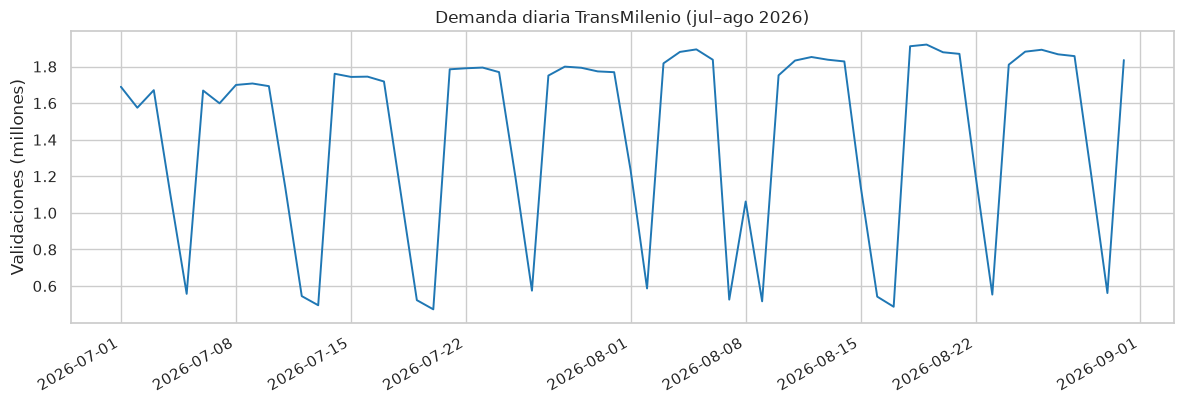
\includegraphics[width=\textwidth]{images/01_serie_temporal_diaria.png}
  \caption{Serie temporal diaria de validaciones.}
\end{minipage}\hfill
\begin{minipage}{0.48\textwidth}
  \centering
  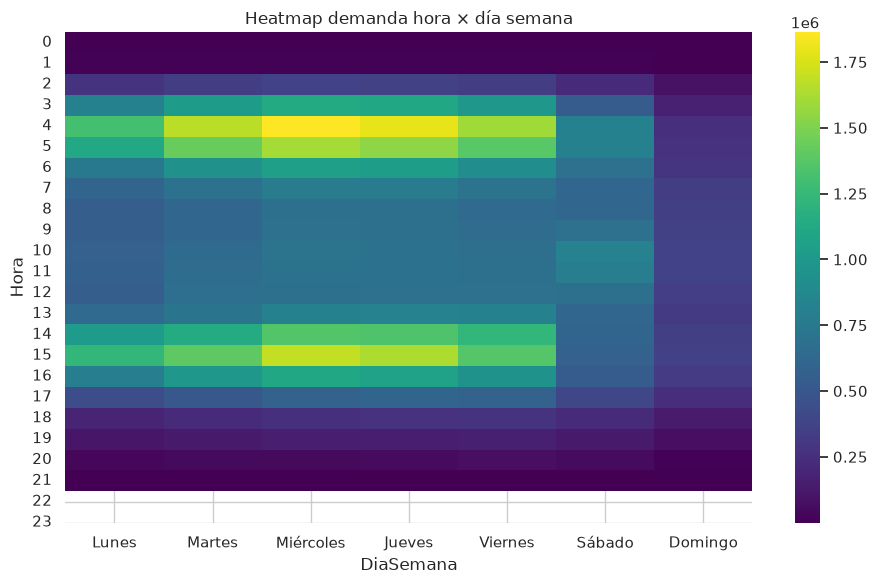
\includegraphics[width=\textwidth]{images/04_heatmap_hora_x_dia_semana.png}
  \caption{Heatmap hora $\times$ día de la semana.}
\end{minipage}
\end{figure}

\begin{figure}[H]
\centering
\begin{minipage}{0.48\textwidth}
  \centering
  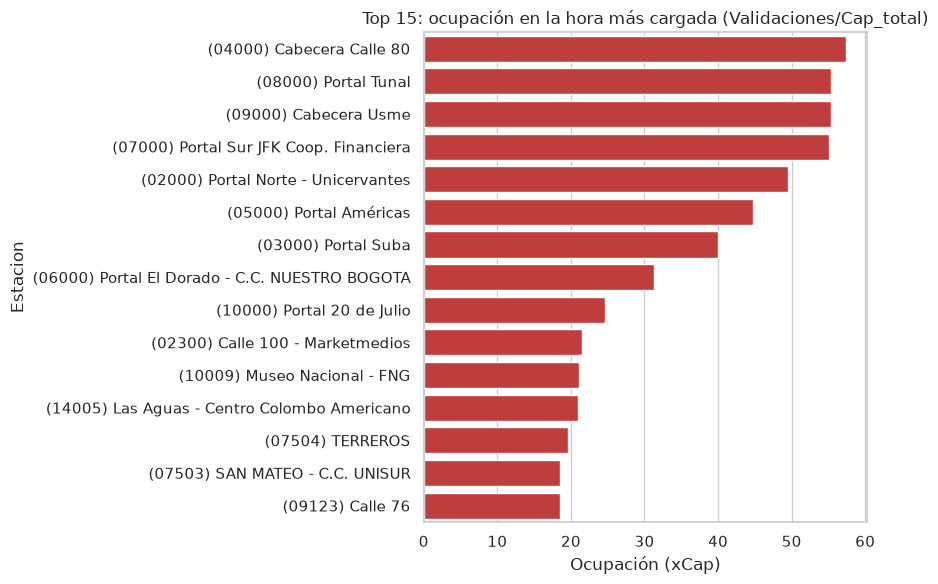
\includegraphics[width=\textwidth]{images/07_top15_ocupacion_pico.png}
  \caption{Top 15 estaciones por ocupación en hora pico.}
\end{minipage}\hfill
\begin{minipage}{0.48\textwidth}
  \centering
  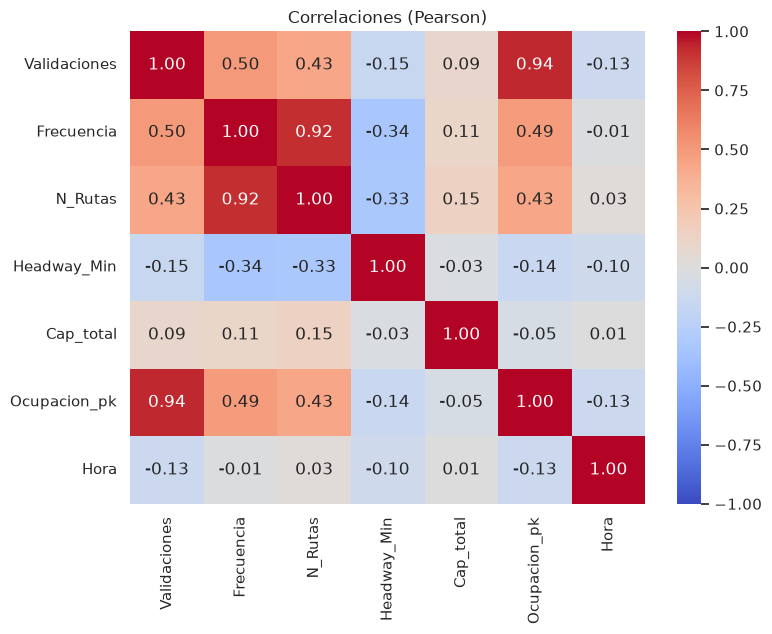
\includegraphics[width=\textwidth]{images/10_matriz_correlacion.png}
  \caption{Matriz de correlación (Pearson).}
\end{minipage}
\end{figure}

%======================================================================
\section{Selección y evaluación de modelos}
\label{sec:modelos}
%----------------------------------------------------------------------
\subsection{Pronóstico de validaciones (base de los módulos)}
Se compara \textbf{Chronos-Bolt-Small} (modelo fundacional de series, zero-shot, descargado de
Hugging Face; tokens numéricos sobre un encoder--decoder estilo T5, entrega pronósticos
probabilísticos con banda q10--q90) contra baselines clásicos mediante \emph{walk-forward} de 5 días
sobre el grid 1,488 h $\times$ 156 estaciones.

\begin{table}[H]
\centering
\caption{Métricas globales del pronóstico (promedio walk-forward 5 días).}
\label{tab:pronostico}
\begin{tabularx}{\textwidth}{lccc}
\toprule
\textbf{Modelo} & \textbf{MAE} & \textbf{RMSE} & \textbf{WMAPE} \\
\midrule
\textbf{Chronos (seleccionado)} & \textbf{56.32} & \textbf{147.32} & \textbf{0.165} \\
Naive\_24 (baseline) & 104.12 & 244.92 & 0.237 \\
\bottomrule
\end{tabularx}
\end{table}

\paragraph{Justificación de Chronos.} Cero riesgo de sobreajuste (62 días por estación), manejo de
series dispersas con ausencias (rellenadas con ceros), cero esfuerzo de despliegue (sin checkpoints
propios), baja latencia en CPU y banda probabilística calibrada auditable frente a `naive\_24`
($\approx$46\% menos MAE y $\approx$40\% menos RMSE).

\subsection{Módulo 1 --- Estimador continuo del tiempo de espera (ETA)}
Cuatro opciones evaluadas en walk-forward: \textbf{A} (`A\_chronos`) pronóstico puro de headway con
Chronos; \textbf{B} (`B\_hist`) tabla histórica ajustada por ocupación ($\times$1.1/$\times$1.3);
\textbf{C} (`C\_blend`) blend $w\cdot A + (1-w)\cdot B$ con peso seleccionado sin fuga;
\textbf{D} (`D\_ratio`) ablación multiplicando por el ratio de congestión sintético.

\begin{table}[H]
\centering
\caption{Comparativa del Módulo 1 (ETA) por opción.}
\label{tab:eta}
\begin{tabularx}{\textwidth}{lcc}
\toprule
\textbf{Opción} & \textbf{MAE (min)} & \textbf{RMSE (min)} \\
\midrule
\textbf{C\_blend (seleccionado)} & \textbf{0.2426} & 1.0854 \\
A\_chronos & 0.2451 & 1.2972 \\
B\_hist & 0.2968 & 0.8859 \\
D\_ratio & 0.4128 & 1.1314 \\
\bottomrule
\end{tabularx}
\end{table}

\paragraph{Lectura.} El blend \textbf{C} gana en MAE. La ablación \textbf{D} (ratio de congestión
sintético) \textbf{empeora} el MAE a 0.413: el ajuste por congestión solo se justifica con telemetría
\textbf{real} (TomTom Traffic) y queda \textbf{desactivado} en esta iteración. En producción
(S08) se recalibraría: $\text{eta\_efectivo} = \text{eta\_base} \times \text{ratio}$.

\subsection{Módulo 2 --- Predictor multiclase de aforo}
La ocupación real se discretiza en tres clases con cuantiles calibrados en \textbf{train}
($l_o = Q60 = 1.479$; $h_i = Q90 = 9.013$). Features: ciclo horario, `dia`, `Es\_Habil` y
`Estacion\_cod`. Ocho clasificadores comparados:

\begin{table}[H]
\centering
\caption{Comparativa de clasificadores de aforo (Módulo 2).}
\label{tab:aforo}
\begin{tabularx}{\textwidth}{lcccc}
\toprule
\textbf{Modelo} & \textbf{accuracy} & \textbf{bal. acc} & \textbf{F1 macro} & \textbf{ROC-AUC ovr} \\
\midrule
\textbf{HistGB (seleccionado)} & \textbf{0.9447} & \textbf{0.9336} & \textbf{0.9408} & 0.9852 \\
LightGBM & 0.9422 & 0.9296 & 0.9373 & 0.9847 \\
XGBoost & 0.9422 & 0.9288 & 0.9372 & \textbf{0.9856} \\
Random Forest & 0.9159 & 0.8813 & 0.9014 & 0.9789 \\
Logistic (baseline) & 0.8120 & 0.6324 & 0.6550 & 0.8851 \\
\bottomrule
\end{tabularx}
\end{table}

Resultado en test (14,178 casos): accuracy \textbf{0.945}; F1 --- Asientos 0.961, De pie 0.904,
Saturado 0.957. El \emph{nowcasting} honesto (misma etiqueta, ocupación real en test) alcanza F1
Saturado 0.876, lo que cuantifica la pérdida esperada al pasar de ocupación real a pronosticada.

\subsection{Módulo 3 --- Motor prescriptivo de recomendación}
Matriz $U(\text{ETA},\,\text{Aforo})$ con umbral recalibrado a 10 min y chequeo de la siguiente
unidad. Se mide la \textbf{fidelidad de preservación de la regla} (AC-03 $\geq 0.80$) y los
falsos positivos de `Abordar` (error de mayor costo).

\begin{table}[H]
\centering
\caption{Comparativa del Módulo 3 (recomendación) sobre el test (12,358 decisiones).}
\label{tab:mod3}
\begin{tabularx}{\textwidth}{lccc}
\toprule
\textbf{Modelo} & \textbf{Fidelidad AC-03} & \textbf{F1 macro} & \textbf{FP Abordar} \\
\midrule
\textbf{Tree (seleccionado)} & \textbf{0.9997} & \textbf{0.9977} & \textbf{0.0000} \\
Random Forest & 0.9997 & 0.9977 & 0.0000 \\
Gradient Boosting & 0.9997 & 0.9977 & 0.0000 \\
HistGB & 0.9992 & 0.9817 & 0.0005 \\
XGBoost & 0.9987 & 0.9611 & 0.0006 \\
\bottomrule
\end{tabularx}
\end{table}

\subsection{Módulo 4 --- Detector de anomalías espacio-temporales}
\textbf{Isolation Forest} (contamination 0.05) entrenado solo sobre el contexto $\leq$ split y
aplicado al test. Umbrales por percentiles: p0.5 $-0.686$, p3.0 $-0.605$. El día más anómalo del
test es 2026-08-31 (fracción de outliers 0.095), consistente con el cierre de señal del periodo.

%======================================================================
\section{Prototipo de baja fidelidad}
\label{sec:wireframes}
%----------------------------------------------------------------------
El flujo de navegación del núcleo requiere \textbf{2 toques} (P1 $\rightarrow$ P2), conforme al
RNF-04. Pantallas principales: selección de servicio/ruta/estación, resultado de aforo (con modo
nocturno automático 18:00--06:00), feedback de un toque y ruta peatonal segura.

\begin{figure}[H]
\centering
\begin{minipage}{0.44\textwidth}
  \centering
  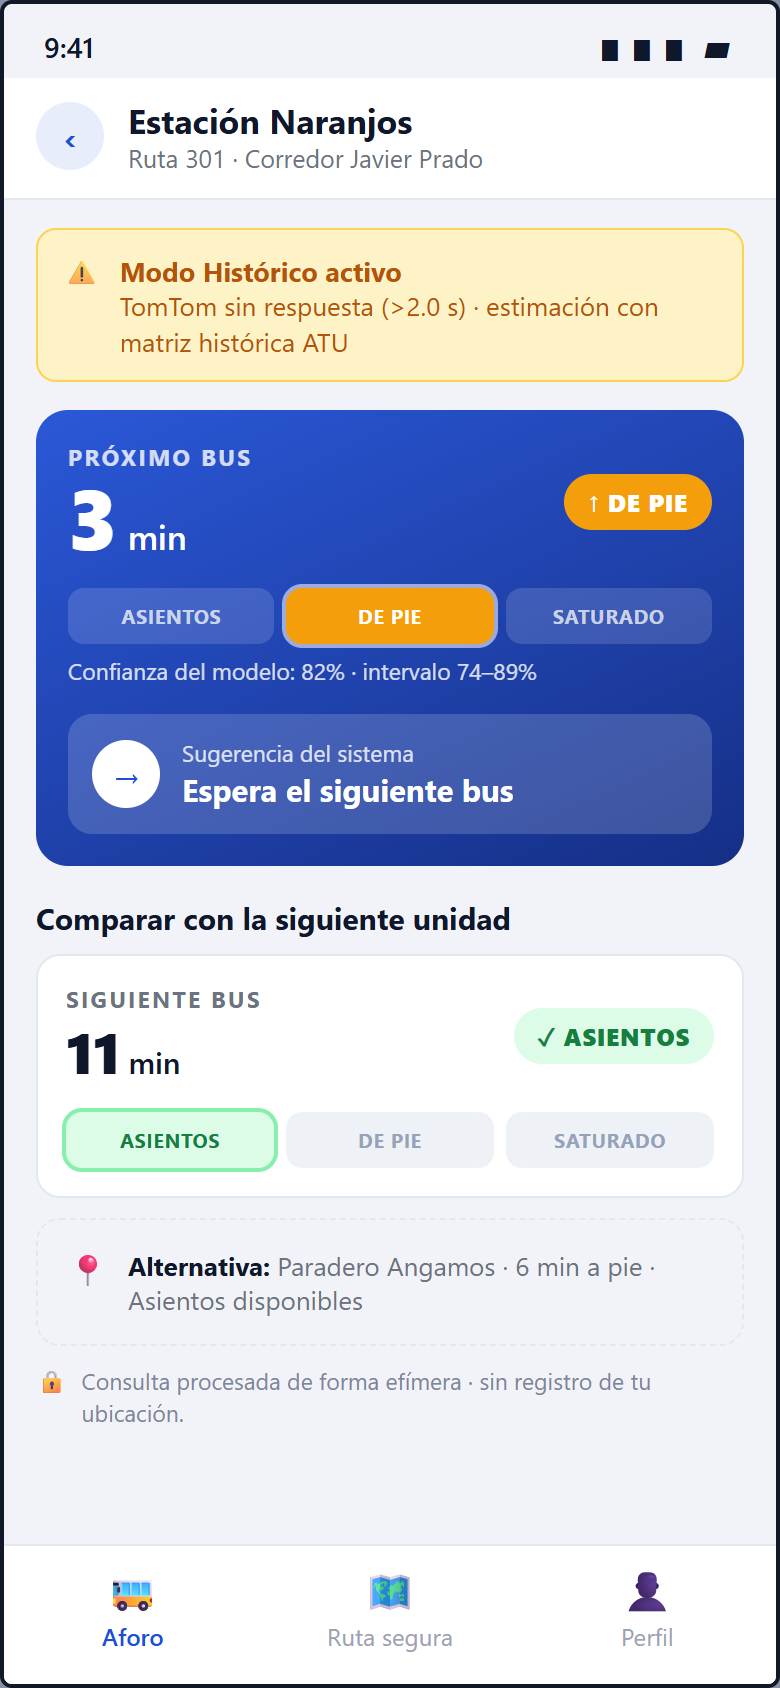
\includegraphics[width=\textwidth]{../img/mobile_02_aforo_resultado.png}
  \caption{Resultado de aforo predictivo (RF-01/02/03).}
\end{minipage}\hfill
\begin{minipage}{0.44\textwidth}
  \centering
  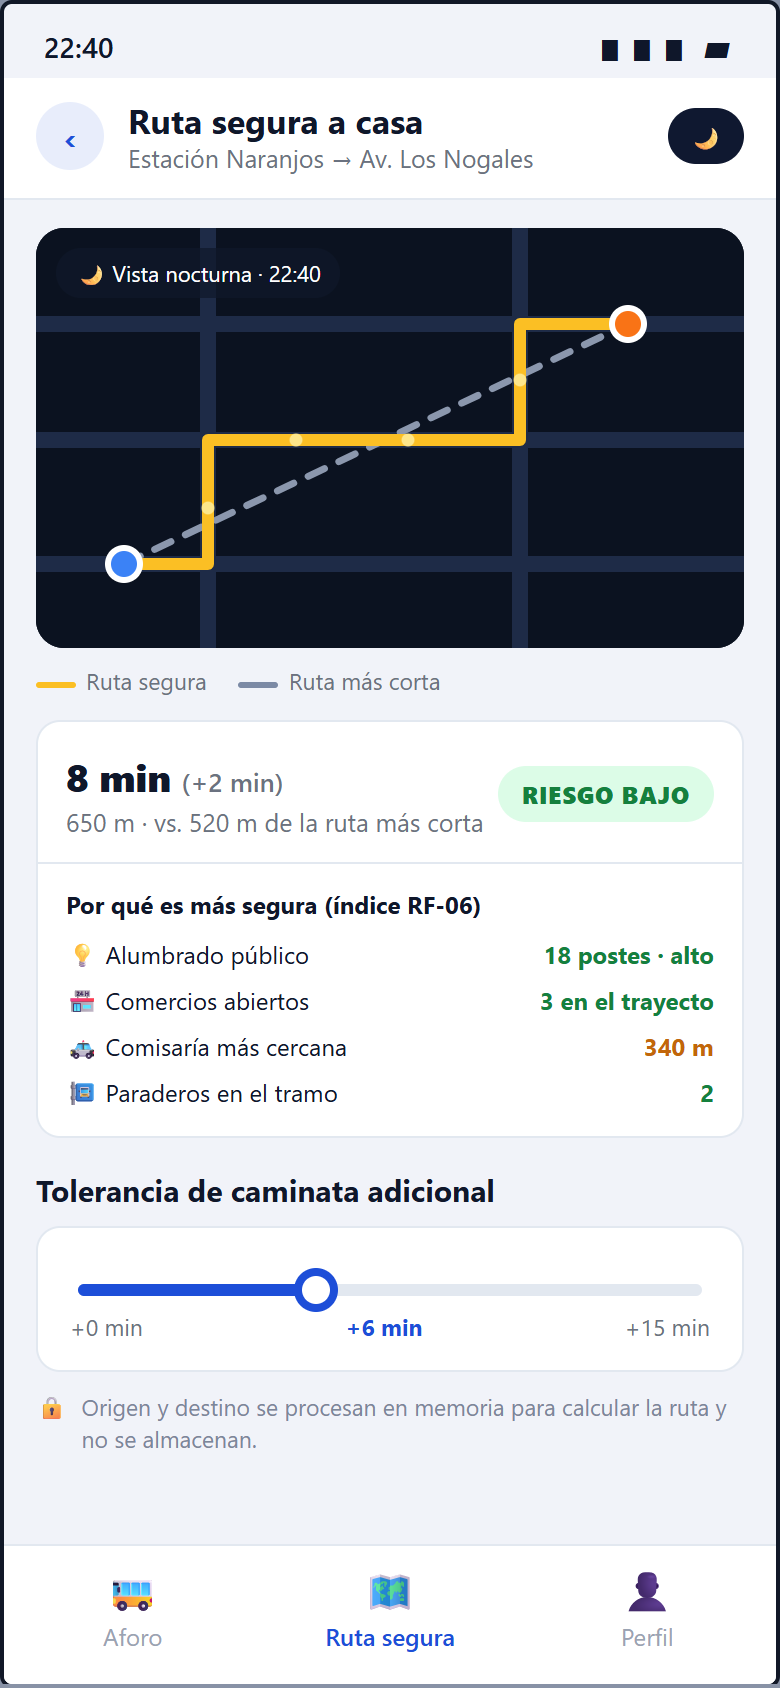
\includegraphics[width=\textwidth]{../img/mobile_05_ruta_peatonal_segura.png}
  \caption{Ruta peatonal segura (RF-06/07/08).}
\end{minipage}
\end{figure}

\paragraph{Trazabilidad requerimiento $\rightarrow$ pantalla.}
\begin{itemize}
  \item RF-01/02/03 y RF-05 $\rightarrow$ pantalla de resultado de aforo (banner de Modo Histórico).
  \item RF-04 $\rightarrow$ pantalla de validación con tres botones de categoría real.
  \item RF-06/07/08 $\rightarrow$ pantalla de ruta peatonal segura (desglose de riesgo, comparativa y
        slider de tolerancia 0--15 min).
  \item RNF-02/04/05 $\rightarrow$ estados de carga, tema oscuro y avisos de procesamiento efímero.
\end{itemize}

%======================================================================
\section{Datasets, diccionarios y pipeline de datos}
\label{sec:datasets}
%----------------------------------------------------------------------
\subsection{Flujo general del pipeline}
\begin{verbatim}
data cruda (TransMilenio / Clima / OSM)            deliveries/week07/data/
        |  process_transmilenio.py . download_*.py
        v
dataset_base.csv (177,944 x 17)                    data/transmilenio/dataset.csv
        |  code/eda/eda_transmilenio.ipynb (limpieza + FE)
        v
dataset_limpio.csv (176,783 x 28)                  data_processed/   <- base de modelado
        |  code/eda/eda_OSM.ipynb
        +-> dataset_osm_estaciones_limpio.csv (156 x 12)
        |  code/scripts/congestion.py (S08: TomTom real)
        +-> congestion_sintetica.csv (232,128 x 7)
        |  code/model/Modelamiento_Preeliminar.ipynb
        +-> pronostico_24h_estaciones.csv (3,480 x 12)
        +-> eval_walkforward_modelos.csv (55 x 5)
        +-> metricas_modelos.csv (2 x 4)
        +-> code/model/outputs/  (comparativas M1/M2/M3)
\end{verbatim}

\subsection{Diccionarios de datos}
Los diccionarios completos se encuentran en \texttt{docs/data\_dictionary}:
\begin{itemize}
  \item Fuentes crudas: \texttt{Data\_Dictionary\_Transmilenio.md}, \texttt{Data\_Dictionary\_Clima.md},
        \texttt{Data\_Dictionary\_OSM.md}.
  \item Procesados y salidas: \texttt{Data\_Dictionary\_Procesados.md},
        \texttt{DatasetDescriptions.md}.
\end{itemize}

\subsection{Claves de unión y trazabilidad}
\begin{table}[H]
\centering
\caption{Relaciones y claves de unión entre datasets.}
\label{tab:claves}
\begin{tabularx}{\textwidth}{lll}
\toprule
\textbf{Desde} & \textbf{Hacia} & \textbf{Clave} \\
\midrule
\texttt{dataset\_limpio} & \texttt{dataset\_osm\_estaciones\_limpio} & \texttt{num\_est} \\
\texttt{dataset\_limpio} & \texttt{clima\_hora\_*.csv} & \texttt{(Fecha, Hora)} \\
\texttt{congestion\_sintetica} & pronóstico / ETA & \texttt{(Estacion, Fecha\_Hora)} \\
\texttt{pronostico\_24h\_estaciones} & contexto histórico & \texttt{(Estacion, Hora\_n)} \\
\bottomrule
\end{tabularx}
\end{table}

\paragraph{Privacidad.} Ningún dataset procesado contiene PII; el número de tarjeta (crudo) es un hash
SHA-256 y no se persiste en \texttt{data\_processed}. La semilla sintética es fija (42) para
reproducibilidad byte a byte.

%======================================================================
\section{Cronograma y próximos pasos}
\label{sec:cronograma}
%----------------------------------------------------------------------
\begin{table}[H]
\centering
\caption{Cronograma de entregables del curso (fases S07--S15).}
\label{tab:cronograma}
\begin{tabularx}{\textwidth}{cl>{\raggedright\arraybackslash}X}
\toprule
\textbf{Semana} & \textbf{Entregable} & \textbf{Responsable principal} \\
\midrule
S07 & \textbf{Integrated Project Definition} (requerimientos, EDA, selección de modelos, datasets) & Elmer (datos), Juan David (modelo), Alessandro (requerimientos/arquitectura) \\
S08 & Examen parcial (sin entrega): ajustar TomTom real y calibrar modelos & Elmer (ingesta), Juan David (modelos) \\
S09 & Prototipo base: API REST, pipeline en vivo, Módulos 3 y 4 & Alessandro (backend), Elmer (pipeline) \\
S10 & \textbf{Prototipo funcional} (frontend, persistencia, métricas vs baselines) & Alessandro (frontend), Juan David (validación) \\
S11 & Eje 2: Módulo peatonal (grafo OSM + costo por riesgo) & Elmer (datos), Juan David (algoritmo), Alessandro (mapa) \\
S12 & Prototipo refinado y casos de estudio (latencia P95 $\leq$ 2 s, \texttt{EvaluationReport.md}) & Elmer (rendimiento), Juan David (evaluación) \\
S13 & Despliegue Cloud \& Docker (URL pública) & Elmer (Docker), Alessandro (cloud) \\
S14 & Video demo final (5--7 min) y Project Page & Alessandro (video), Juan David (informe final) \\
S15 & \textbf{Entrega final} \& presentación pública + README definitivo & Todo el equipo \\
\bottomrule
\end{tabularx}
\end{table}

\subsection{Próximos pasos técnicos (Fase 2, S08--S10)}
\begin{itemize}
  \item Integrar \textbf{TomTom Traffic} real y recalibrar sin reentrenar: $\text{eta\_efectivo} =
        \text{eta\_base} \times \text{ratio}$ (desactiva la ablación D sintética).
  \item Serializar los artefactos ML (Chronos zero-shot, HistGB, Tree) y diseñar el esquema
        OpenAPI/Swagger del backend FastAPI.
  \item Implementar la cascade de inferencia con latencia P95 $\leq$ 2 s y el modo resiliente RF-05.
  \item Persistencia (PostgreSQL/DuckDB) y primer frontend funcional.
  \item Validar el módulo peatonal (grafo OSM, índice de riesgo) en S11.
\end{itemize}

%======================================================================
\section{Referencias}
\label{sec:referencias}
%----------------------------------------------------------------------
\begin{itemize}
  \item INEI (2025). \emph{Percepción de la Inseguridad Ciudadana y Victimización en Áreas Urbanas de
        Lima Metropolitana}. \url{https://www.inei.gob.pe/estadisticas/indice-tematico/seguridad-ciudadana/}
  \item ATU (2026). \emph{Hackathon 2026}.
        \url{https://www.gob.pe/institucion/atu/noticias/atu-lanza-la-hackathon-2026}
  \item ProTransporte \& ATU. \emph{Portal de Datos Abiertos del Sistema Integrado de Transporte}.
        \url{https://sistemas.protransporte.gob.pe/DatosAbiertos/}
  \item TransMilenio (Bogotá). \emph{Datos abiertos del operador}.
        \url{https://www.transmilenio.gov.co/datosAbiertos/}
  \item TomTom Traffic API. \url{https://docs.tomtom.com/traffic-api/}
  \item Amazon Science. \emph{Chronos-Bolt (pronóstico de series)}.
        \url{https://github.com/amazon-science/chronos-forecasting}
\end{itemize}

\subsection{Documentación interna del repositorio}
\begin{itemize}
  \item \texttt{deliveries/week07/docs/Requirements.md} --- especificación de requerimientos (RF/RNF, AC).
  \item \texttt{deliveries/week07/docs/DataAnalysis.md} --- EDA (fuentes, preprocesamiento, hallazgos).
  \item \texttt{deliveries/week07/docs/ModelSelection.md} --- selección/justificación de modelos y resultados.
  \item \texttt{deliveries/week07/docs/Wireframes.md} --- wireframes de baja fidelidad.
  \item \texttt{deliveries/week07/docs/data\_dictionary/} --- diccionarios de datos (crudos y procesados).
  \item \texttt{deliveries/week07/code/download/Guia.md} --- guía técnica de descarga/ingesta.
\end{itemize}

\end{document}